\documentclass[12pt]{report}
\usepackage[utf8]{inputenc}
\usepackage[russian]{babel}
%\usepackage[14pt]{extsizes}
\usepackage{listings}
\usepackage{graphicx}
\usepackage{amsmath,amsfonts,amssymb,amsthm,mathtools} 
\usepackage{pgfplots}
\usepackage{filecontents}
\usepackage{indentfirst}
\usepackage{eucal}
\usepackage{amsmath}
\usepackage{enumitem}
\frenchspacing

\usepackage{indentfirst} % Красная строка


%\usetikzlibrary{datavisualization}
%\usetikzlibrary{datavisualization.formats.functions}

\usepackage{amsmath}




% Для листинга кода:
\lstset{ %
language=haskell,                 % выбор языка для подсветки (здесь это С)
basicstyle=\small\sffamily, % размер и начертание шрифта для подсветки кода
numbers=left,               % где поставить нумерацию строк (слева\справа)
numberstyle=\tiny,           % размер шрифта для номеров строк
stepnumber=1,                   % размер шага между двумя номерами строк
numbersep=5pt,                % как далеко отстоят номера строк от подсвечиваемого кода
showspaces=false,            % показывать или нет пробелы специальными отступами
showstringspaces=false,      % показывать или нет пробелы в строках
showtabs=false,             % показывать или нет табуляцию в строках
frame=single,              % рисовать рамку вокруг кода
tabsize=2,                 % размер табуляции по умолчанию равен 2 пробелам
captionpos=t,              % позиция заголовка вверху [t] или внизу [b] 
breaklines=true,           % автоматически переносить строки (да\нет)
breakatwhitespace=false, % переносить строки только если есть пробел
escapeinside={\#*}{*)}   % если нужно добавить комментарии в коде
}

\usepackage[left=2cm,right=2cm, top=2cm,bottom=2cm,bindingoffset=0cm]{geometry}
% Для измененных титулов глав:
\usepackage{titlesec, blindtext, color} % подключаем нужные пакеты
\definecolor{gray75}{gray}{0.75} % определяем цвет
\newcommand{\hsp}{\hspace{20pt}} % длина линии в 20pt
% titleformat определяет стиль
\titleformat{\chapter}[hang]{\Huge\bfseries}{\thechapter\hsp\textcolor{gray75}{|}\hsp}{0pt}{\Huge\bfseries}


% plot
\usepackage{pgfplots}
\usepackage{filecontents}
\usetikzlibrary{datavisualization}
\usetikzlibrary{datavisualization.formats.functions}

\begin{document}
%\def\chaptername{} % убирает "Глава"
\thispagestyle{empty}
\begin{titlepage}
	\noindent \begin{minipage}{0.15\textwidth}
	
\includegraphics[width=\linewidth]{b_logo}
	\end{minipage}
	\noindent\begin{minipage}{0.9\textwidth}\centering
		\textbf{Министерство науки и высшего образования Российской Федерации}\\
		\textbf{Федеральное государственное бюджетное образовательное учреждение высшего образования}\\
		\textbf{~~~«Московский государственный технический университет имени Н.Э.~Баумана}\\
		\textbf{(национальный исследовательский университет)»}\\
		\textbf{(МГТУ им. Н.Э.~Баумана)}
	\end{minipage}
	
	\noindent\rule{18cm}{3pt}
	\newline\newline
	\noindent ФАКУЛЬТЕТ $\underline{\text{«Информатика и системы управления»}}$ \newline\newline
	\noindent КАФЕДРА $\underline{\text{«Программное обеспечение ЭВМ и информационные технологии»}}$\newline\newline\newline\newline\newline
	
	
	\begin{center}
		\noindent\begin{minipage}{1.3\textwidth}\centering
			\Large\textbf{  Отчёт по лабораторной работе №4}\newline
			\textbf{по дисциплине "Анализ алгоритмов"}\newline\newline
		\end{minipage}
	\end{center}
	
	\noindent\textbf{Тема} $\underline{\text{Параллельное умножение матриц}}$\newline\newline
	\noindent\textbf{Студент} $\underline{\text{Романов А.В.}}$\newline\newline
	\noindent\textbf{Группа} $\underline{\text{ИУ7-53Б}}$\newline\newline
	\noindent\textbf{Оценка (баллы)} $\underline{\text{~~~~~~~~~~~~~~~~~~~~~~~~~~~}}$\newline\newline
	\noindent\textbf{Преподаватели} $\underline{\text{Волкова Л.Л., Строганов Ю.В.}}$\newline\newline\newline
	
	\begin{center}
		\vfill
		Москва~---~\the\year
		~г.
	\end{center}
\end{titlepage}


\tableofcontents

\newpage
\chapter*{Введение}
\addcontentsline{toc}{chapter}{Введение}


Задачи лабораторной работы:

\begin{enumerate}
	\item test
\end{enumerate}

\chapter{Аналитическая часть}


\section{Стандартный алгоритм}

\section{Алгоритм Копперсмита -- Винограда}


\section{Вывод}
	Вывод
\clearpage

\chapter{Конструкторская часть}

\section{Схемы алгоритмов}


\begin{figure}[h]
	\centering
	%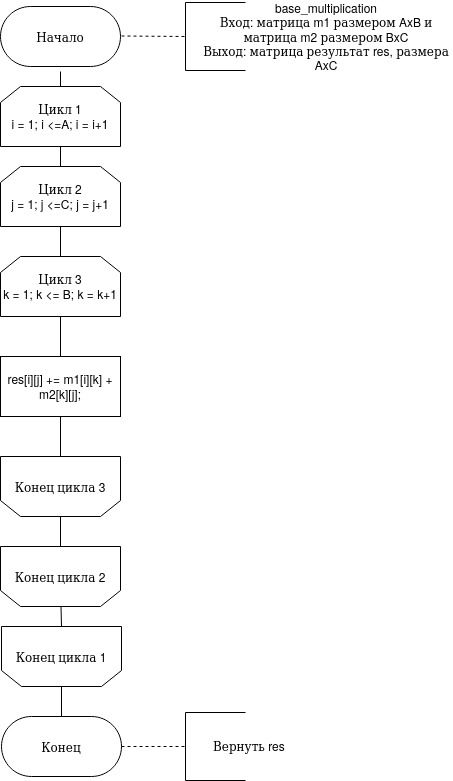
\includegraphics[width=1\linewidth]{base.jpg}
	\caption{Схема стандартного алгоритма умножения матриц}
	\label{fig:mpr}
\end{figure}

\begin{figure}[h]
	\centering
	%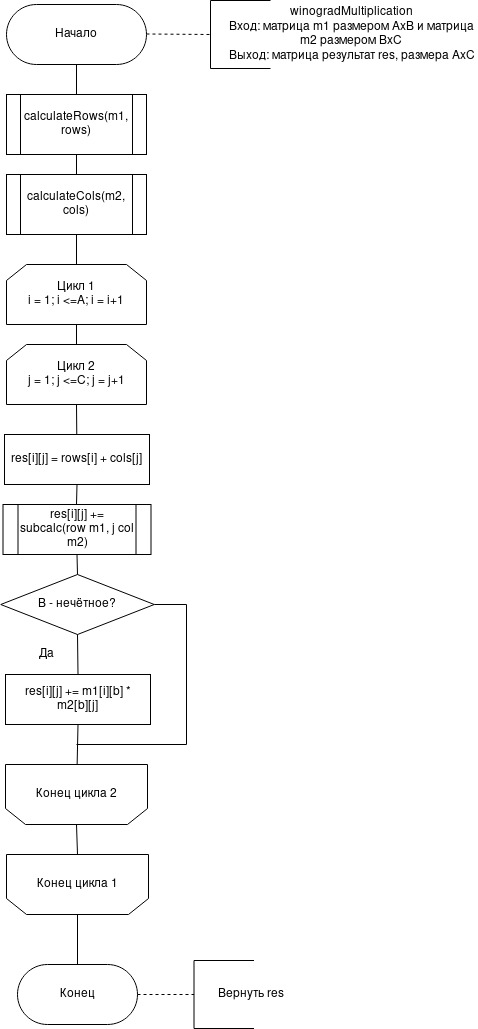
\includegraphics[scale=0.6]{winograd_0.jpg}
	\caption{Схема алгоритма Копперсмита -- Винограда}
	\label{fig:mpr}
\end{figure}

\begin{figure}[h]
	\centering
	%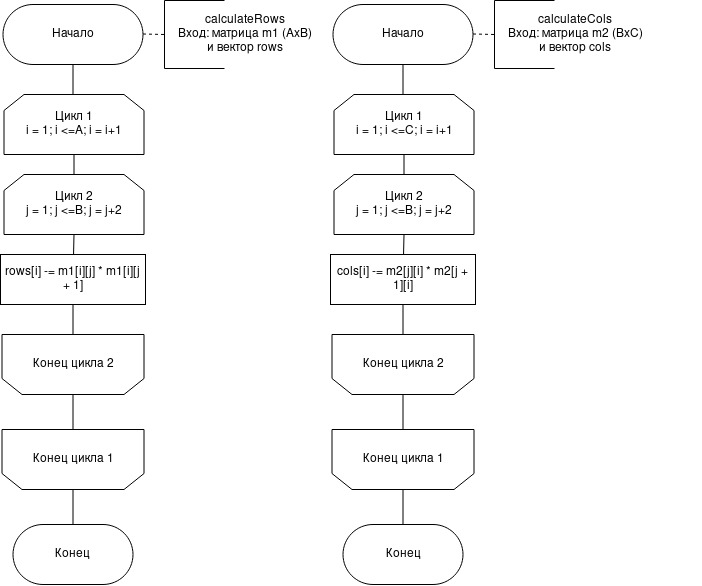
\includegraphics[scale=0.8]{winograd_1.jpg}
	\caption{Схема функций алгоритма Копперсмита -- Винограда}
	\label{fig:mpr}
\end{figure}

\begin{figure}[h]
	\centering
	%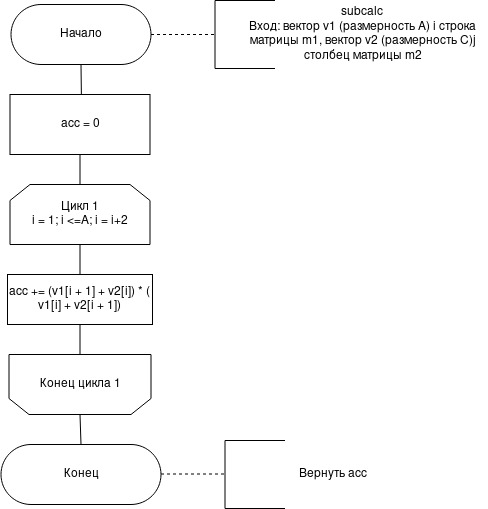
\includegraphics[scale=1]{winograd_2.jpg}
	\caption{Схема функций алгоритма Копперсмита -- Винограда}
	\label{fig:mpr}
\end{figure}

\begin{figure}[h]
	\centering
	%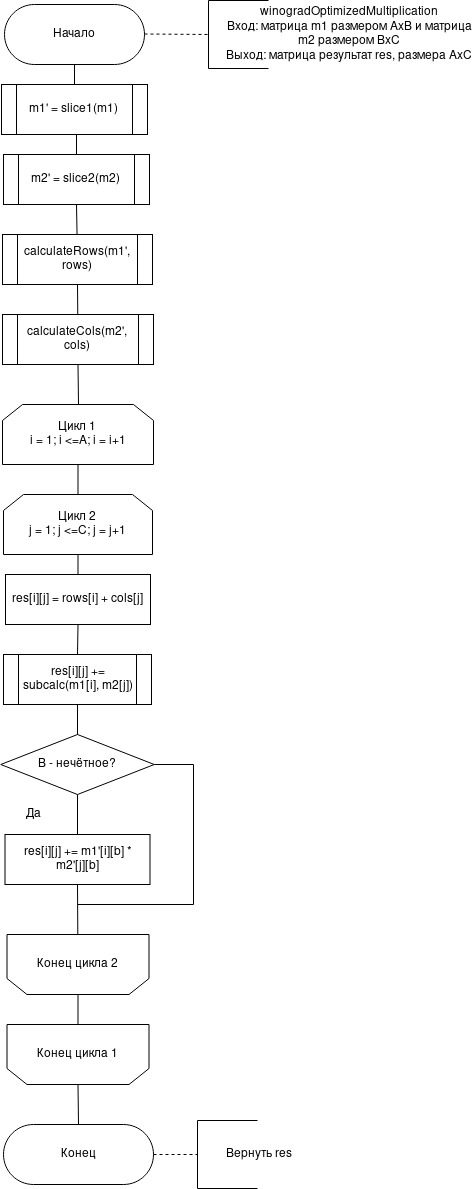
\includegraphics[width=0.5\linewidth]{winograd_opt_0.jpg}
	\caption{Схема оптимизированного алгоритма Копперсмита -- Винограда}
	\label{fig:mpr}
\end{figure}

\begin{figure}[h]
	\centering
	%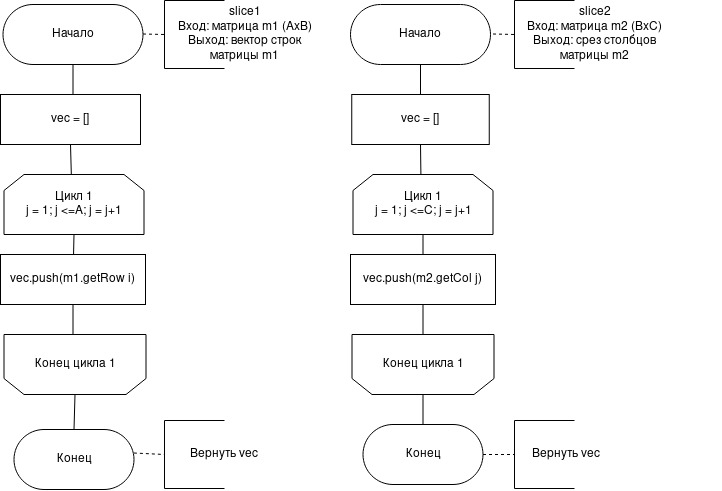
\includegraphics[scale=0.8]{winograd_opt_1.jpg}
	\caption{Схема функций оптимизированного алгоритма Копперсмита -- Винограда}
	\label{fig:mpr}
\end{figure}


\section{Вывод}
	На основе теоретических данных, полученных из аналитического раздела, были построены схемы обоих алгоритмов умножения матриц.  Оценены их трудоёмкости в лучшем и худшем случаях.

\chapter{Технологическая часть}

В данном разделе приведены средства реализации и листинги кода.

\section{Требование к ПО}

К программе предъявляется ряд требований:

\begin{itemize}

	\item 123

\end{itemize}

\section{Средства реализации}
Для реализации ПО я выбрал язык программирования Haskell \cite{C}. Данный выбор обусловлен ???

\section{Реализация алгоритмов}

В листингах 3.1 - 3.4 приведена реализация алгоритмов перемножения матриц.

\begin{lstlisting}[label=some-code,caption=Функция умножения матриц обычным способом, language=C]
void base_multiplication(args_t *args) {
	for (int i = 0; i < N; i++) {
		for (int j = 0; j < K; j++) {
			args->res[i][j] = 0;
			for (int k = 0; k < M; k++) {
				args->res[i][j] += args->m1[i][k] * args->m2[k][j];
			}
		}
	}
}
\end{lstlisting}

\begin{lstlisting}[label=some-code,caption=Функция умножения матриц параллельно. Способ №1,language=C]
void *parallel_multiplication1(void *args) {
	pthread_args_t *argsp = (args_t *)args;

	int row_start = argsp->tid * (argsp->size / argsp->cnt_threads);
	int row_end = (argsp->tid + 1) * (argsp->size / argsp->cnt_threads);

	for (int i = row_start; i < row_end; i++) {
		for (int j = 0; j < K; j++) {
			argsp->mult_args->res[i][j] = 0;
			for (int k = 0; k < M; k++) {
				argsp->mult_args->res[i][j] += argsp->mult_args->m1[i][k] * argsp->mult_args->m2[k][j];
			}
		}
	}

	return NULL;
}

\end{lstlisting}

\begin{lstlisting}[label=some-code,caption=Функция умножения матриц параллельно. Способ №2,language=C]
void *parallel_multiplication2(void *args) {
	pthread_args_t *argsp = (args_t *)args;

	int col_start = argsp->tid * (argsp->size / argsp->cnt_threads);
	int col_end = (argsp->tid + 1) * (argsp->size / argsp->cnt_threads);

	for (int i = 0; i < N; i++) {
		for (int j = col_start; j < col_end; j++) {
			argsp->mult_args->res[i][j] = 0;
			for (int k = 0; k < M; k++) {
				argsp->mult_args->res[i][j] += argsp->mult_args->m1[i][k] * argsp->mult_args->m2[k][j];
			}
		}
	}

	return NULL;
}

\end{lstlisting}

\section{Тестовые данные}

В таблице~\ref{tabular:test_rec} приведены тесты для функций, реализующих параллельное и обычное умножение матриц. Все тесты пройдены успешно.

\begin{table}[h!]
	\begin{center}
		\begin{tabular}{c@{\hspace{7mm}}c@{\hspace{7mm}}c@{\hspace{7mm}}c@{\hspace{7mm}}c@{\hspace{7mm}}c@{\hspace{7mm}}}
			\hline
			Первая матрица & Вторая матрица & Ожидаемый результат \\ \hline
			\vspace{4mm}
			$\begin{pmatrix}
			1 & 2 & 3\\
			1 & 2 & 3\\
			1 & 2 & 3
			\end{pmatrix}$ &
			$\begin{pmatrix}
			1 & 2 & 3\\
			1 & 2 & 3\\
			1 & 2 & 3
			\end{pmatrix}$ &
			$\begin{pmatrix}
			6 & 12 & 18\\
			6 & 12 & 18\\
			6 & 12 & 18
			\end{pmatrix}$ \\
			\vspace{2mm}
			\vspace{2mm}
			$\begin{pmatrix}
			1 & 2 & 2\\
			1 & 2 & 2
			\end{pmatrix}$ &
			$\begin{pmatrix}
			1 & 2\\
			1 & 2\\
			1 & 2
			\end{pmatrix}$ &
			$\begin{pmatrix}
			5 & 10\\
			5 & 10
			\end{pmatrix}$ \\
			\vspace{2mm}
			\vspace{2mm}
			$\begin{pmatrix}
			2
			\end{pmatrix}$ &
			$\begin{pmatrix}
			2
			\end{pmatrix}$ &
			$\begin{pmatrix}
			4
			\end{pmatrix}$ \\
			\vspace{2mm}
			\vspace{2mm}
			$\begin{pmatrix}
			1 & -2 & 3\\
			1 & 2 & 3\\
			1 & 2 & 3
			\end{pmatrix}$ &
			$\begin{pmatrix}
			-1 & 2 & 3\\
			1 & 2 & 3\\
			1 & 2 & 3
			\end{pmatrix}$ &
			$\begin{pmatrix}
			0 & 4 & 6\\
			4 & 12 & 18\\
			4 & 12 & 18
			\end{pmatrix}$\\
			\vspace{2mm}
			\vspace{2mm}
		\end{tabular}
	\end{center}
	\caption{\label{tabular:test_rec} Тестирование функций}
\end{table}

\section{Вывод}

Вывод 3

\chapter{Исследовательская часть}

\section{Технические характеристики}

Ниже приведены технические характеристики устройства, на котором было проведено тестирование ПО:

\begin{itemize}
	\item Операционная система: Debian \cite{debian} Linux \cite{linux} 11 <<bullseye>> 64-bit.
	\item Оперативная память: 12 GB.
	\item Процессор: Intel(R) Core(TM) i5-3550 CPU @ 3.30GHz
\cite{i5}.

\end{itemize}

\section{Время выполнения алгоритмов}
Тики
\newline

В таблицах 4.1 и 4.2 представлены замеры времени работы для

\begin{table} [h!]
	\caption{Таблица времени выполнения алгоритмов (в секундах)}
	\begin{center}
		\begin{tabular}{|c c c c c|} 
		 	\hline
			Размер матрицы & С & ТС & КВ & ОКВ \\  
		 	\hline
		 	100 & 0.482 & 0.120 & 0.169 & 0.158 \\
		 	\hline
		 	200 & 3.998 & 0.947 & 1.312 & 1.253 \\
		 	\hline
			300 & 13.526 & 3.364 & 4.478 & 4.063 \\
			\hline
			400 & 34.330 & 7.521 & 11.319 & 9.909 \\
			\hline
			500 & NaN & 14.913 & 22.427 & 19.357 \\
			\hline
			600 & NaN & 26.448 & 39.292 & 33.265 \\
			\hline
		\end{tabular}
	\end{center}
\end{table}


\section{Вывод}

\chapter*{Заключение}
\addcontentsline{toc}{chapter}{Заключение}

В рамках данной лабораторной работы:

\begin{enumerate}
	\item тест
\end{enumerate}


\addcontentsline{toc}{chapter}{Литература}

\bibliographystyle{utf8gost705u}  % стилевой файл для оформления по ГОСТу

\bibliography{51-biblio}          % имя библиографической базы (bib-файла)


\end{document}
